\chapter{Introduction}
\label{chap:intro}
\begin{shortAbstract}
A short abstract for the upcoming chapter
\end{shortAbstract}


\section{Illustration Example}

\subsection{A subsection just for fun}

Sorry I won't write your PhD here ;) This small text just to mention that this style supports writing with accents such as in french words (thse, dfinir, ...). Also I put here a simple way to include an image. This is standard latex. For pdflatex compilation, the extension of the images is jpg. For latex compilation, this is ps or eps. The base folder containing images is set in formatAndDefs.tex, as well as the default extensions added to the image names.

\begin{figure}[!htbp]
  \begin{center}
    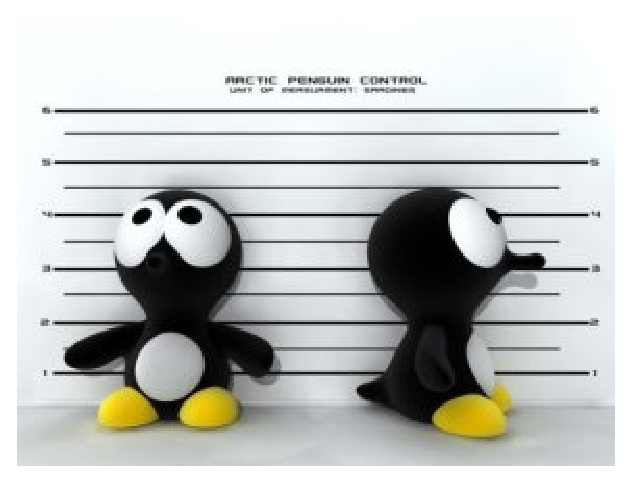
\includegraphics[width=0.9\textwidth]{Chapter1/arctic_control}
  \end{center}
  \caption{A nice image...}
  \label{fig:jolieImage}
\end{figure}

\section{An equation}

Just to show argmin and partial derivative commands.
First, we want to obtain a registration method which is as independent as possible w.r.t. the setting of its parameters. This setting, done by the clinician, indeed needs to be minimal while guaranteeing a robust result. We therefore propose registration methods allowing to better control the obtained transformation, using outlier rejection techniques or locally affine transformations.First, we want to obtain a registration method which is as independent as possible w.r.t. the setting of its parameters. This setting, done by the clinician, indeed needs to be minimal while guaranteeing a robust result. We therefore propose registration methods allowing to better control the obtained transformation, using outlier rejection techniques or locally affine transformations.First, we want to obtain a registration method which is as independent as possible w.r.t. the setting of its parameters. This setting, done by the clinician, indeed needs to be minimal while guaranteeing a robust result. We therefore propose registration methods allowing to better control the obtained transformation, using outlier rejection techniques or locally affine transformations.First, we want to obtain a registration method which is as independent as possible w.r.t. the setting of its parameters. This setting, done by the clinician, indeed needs to be minimal while guaranteeing a robust result. We therefore propose registration methods allowing to better control the obtained transformation, using outlier rejection techniques or locally affine transformations.
First, we want to obtain a registration method which is as independent as possible w.r.t. the setting of its parameters. This setting, done by the clinician, indeed needs to be minimal while guaranteeing a robust result. We therefore propose registration methods allowing to better control the obtained transformation, using outlier rejection techniques or locally affine transformations.First, we want to obtain a registration method which is as independent as possible w.r.t. the setting of its parameters. This setting, done by the clinician, indeed needs to be minimal while guaranteeing a robust result. We therefore propose registration methods allowing to better control the obtained transformation, using outlier rejection techniques or locally affine transformations.
Regularization:

\begin{equation}
  \pd{T}{t} = \Delta T
\end{equation}

\section{An other section}

Showing a great bullet list environme